\subsection{a)}
For a steady state the following conditions must hold
$$0 = a - (b+1)u + u^2v$$
$$0 = bu - u^2v$$

Then simply find the steady state by calculating,
$$0 = a-(b+1)u +bu$$
$$0 = a - u$$
$$u = a$$

$$0 = ba - a^2v$$
$$v = \frac{b}{a}$$

The steady state found is,
$$(u^*, v^*)=\left(a,\frac{b}{a}\right)$$

To find if the steady state is stable the jacobian is first calculated
$$J^* = \left(
\begin{array}{cc}
    b-1 & a^2 \\
    -b  & -a^2
\end{array}
\right)$$

For the steady state to be stable the following conditions must be true

$$Tr(J^*) < 0$$
$$Det(J^*) > 0$$
Inserting the given values $a=3$, $b=8$ we get
$$Tr(J^*) = -2 < 0$$
$$Det(J^*) = 9 > 0$$
Thus the steady state is stable.

For the system to exhibit diffusion driven instability the following conditions must also hold

$$D_v \frac{\partial f}{\partial u} + \frac{\partial g}{\partial v} < 0$$
$$(D_v \frac{\partial f}{\partial u}+ \frac{\partial g}{\partial v})^2 - 4D_v Det(J^*) > 0$$

Inserting the values for $a, b$ and $(u^*, v^*)$, the first equation evaluates to

$$D_v > \frac{9}{7}$$

and the second to
$$D_v > \frac{81}{49} + \sqrt{\left(\frac{81}{49}\right)^2 - \frac{81}{49}} = 2.69$$
$$D_v < \frac{81}{49} - \sqrt{\left(\frac{81}{49}\right)^2 - \frac{81}{49}} = 0.61$$

Thus for the system to exhibit diffusion driven instability $D_v > 2.69$, since $0.61 < \frac{9}{7}$.


\subsection{b)}

\begin{figure}[h]
    \centering
    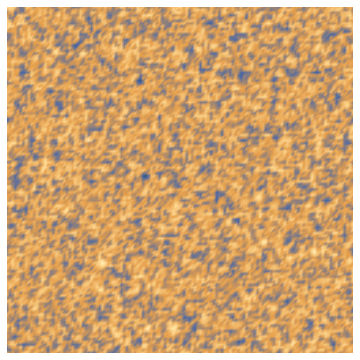
\includegraphics[width=0.45\textwidth]{img/2bd23transient.png}
    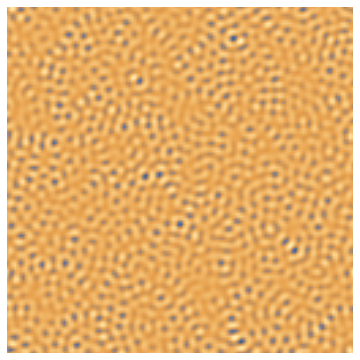
\includegraphics[width=0.45\textwidth]{img/2bd23.png}
  \caption{System simulated with $D_v=2.3$. The picture to the left shows the system in the transient state after 25 time steps, and the picture to the right shows the system after reaching the steady state.}
\end{figure}

\begin{figure}[h]
    \centering
    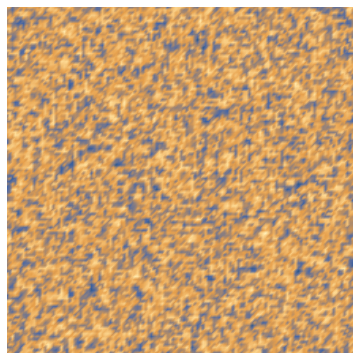
\includegraphics[width=0.45\textwidth]{img/2bd3transient.png}
    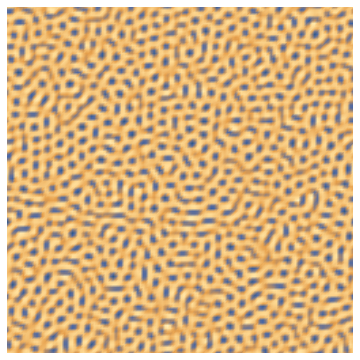
\includegraphics[width=0.45\textwidth]{img/2bd3.png}
  \caption{System simulated with $D_v=3$. The picture to the left shows the system in the transient state after 25 time steps, and the picture to the right shows the system after reaching the steady state.}
\end{figure}

\begin{figure}[h]
    \centering
    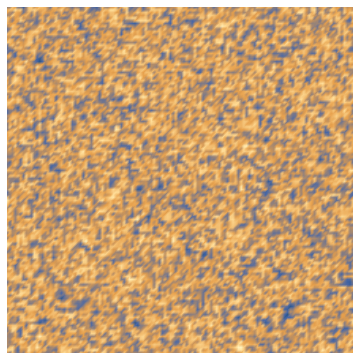
\includegraphics[width=0.45\textwidth]{img/2bd5transient.png}
    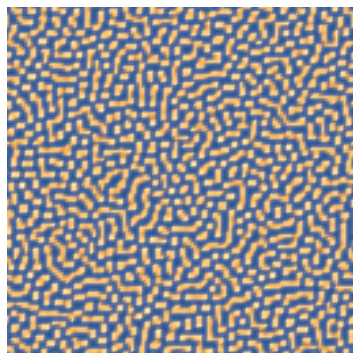
\includegraphics[width=0.45\textwidth]{img/2bd5.png}
  \caption{System simulated with $D_v=5$. The picture to the left shows the system in the transient state after 25 time steps, and the picture to the right shows the system after reaching the steady state.}
\end{figure}

\begin{figure}[h]
    \centering
    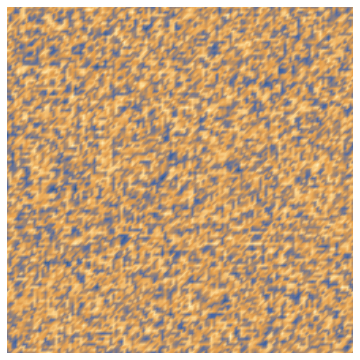
\includegraphics[width=0.45\textwidth]{img/2bd9transient.png}
    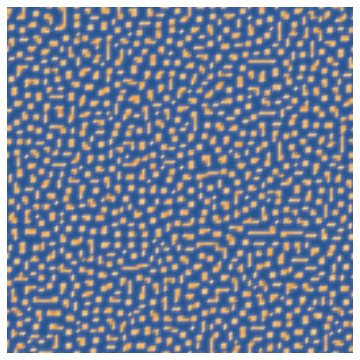
\includegraphics[width=0.45\textwidth]{img/2bd9.png}
  \caption{System simulated with $D_v=9$. The picture to the left shows the system in the transient state after 25 time steps, and the picture to the right shows the system after reaching the steady state.}
\end{figure}
